\chapter{Building PET}
PET is a Power Estimation Tool that provides guided information about power
usage for new architectures, and represents a major piece of our problem
solution. The following chapters will describe how it works along with it's
strengths and weaknesses.

\noindent Source code for PET lives at github.com and can be checked out with
\begin{lstlisting}[language=bash]
git checkout https://github.com/terjr/thesis.git
\end{lstlisting}

\section{Concept}
The goal for PET and this project is to ultimatly estimate power usage and thus
also energy efficiency of still not yet implemented computer architectures. A
such approach will of course reside well within the term "estimation" and will
doubtly reach the correct numbers. Never the less, PET is built by measuring
real hardware with great detail, capturing discrete events and assigning each
event a certain amount of energy consumption.

As depicted in \autoref{fig:workflow}, when selected events have been weighted,
one can run the test program though a simulator set up to act as the new
hardware.  The simulator will generate a tracelog containing the weighted
events, and PET can then apply the numbers. From this workflow, PET can produce
a data set containing power consumption distributed over the simulation
lifetime.  As noted, the new hardware will be weighted equally of a chosen
existing hardware, so so this method requires a certain similarity beteen the
new and the old hardware. In general, all traditional architectures contains
equal principles of function, and is thus mappable to each other, but accuracy
will of course differ as hardware differs in design, applied voltage, clock
speed and process technology.

\begin{figure}
    \includegraphics[width=0.9\textwidth]{figs/pet-workflow-gv.pdf}
    \caption{Workflow using PET}
    \label{fig:workflow}
\end{figure}

When estimating power usage for new architectures, it is hard to tell exactly
how to chose events and how expensive each event is. Therefore, we have to
assume that the new architecture is comparable to an old architecture, and thus
we can use the same power estimation numbers to give a new estimate.

\section{Methodology}

\subsection{Design Choices}
\label{subsec:design_choises}
The first choices made on how PET should be designed was to decide whether it
should be a standalone program or incorporated into an existing simulator.
Hundreds of computer architecture simulators exists, all with strengths and
weknesses. Often, simulators only supports a small set of architectures, memory
systems and CPU models, and they are only good at simulating one specific
combination.

It is desirable to estimate energy consumption on literally all types of
compututing systems, ranging from large-size clusters to embedded systems. To
provide this flexibility it was decided to write the tool as simulator agnostic
as possible, tracking \emph{simulator events} rather than executed instructions.
A simulator event is defined as a unit of work that uses a specified amount of
energy, and increases modelled energy consumption to the simulated time.

%\begin{center}
%    \begin{tabular}{|l|l|}
%        \hline
%        L1D & L1 data hit\\
%        \hlinke
%    \end{tabular}
%\end{center}

gem5 was used as a basis for development and the only simulation front-end
implemented.




- ARM support (Sniper has not)

QEMU -- feil abstraksjonsnivå/formål
McPat - multicore, power AND AREA???? Optimizer
gem5 is flexible because
    - it is easy to add new processor architectures
    - memory system
=> in-house experience

LLVM traces?


\section{Architecture}

Modern computer science emphasize parallelism as a highly important property in
order to achieve speed on multicore processors. As the size of the log files
which PET has to parse can easily be 10s of gigabytes large, PET has to be
designed with performance in mind. This means that PET must be lightweight and
parallel in order to be fast, while it must maintain correctness and be easy to
use.

Due to memory constraints on commonly available computers, it is not feasible to
read the entire log file into memory and then start parsing. It would also make
the reading step a serial part of the program, which hinders parallelism. It
will also be a bad idea to read one line, parse it, weight it and apply it to
the grand total, as it would be an entirely serial process.

\subsection{Overview}

\begin{figure}[ht]
    \includegraphics[width=0.9\textwidth]{figs/pet-pipeline-gv.pdf}
    \caption{How PET works}
    \label{fig:pipeline}
\end{figure}

In order to maintain good speed while still keeping the PET source code
readable, we have looked at different ways of chewing through large data sets.
The final implementation of PET follows a scheme borrowing ideas from the
producer-consumer patterb as explained by Gamma et. al. in \cite{designpatterns}
and the MapReduce algorithm \cite{dean2008mapreduce}. As depicted in
\autoref{fig:pipeline}, this scheme makes it rather easy to let a producer read
the lines from the log file into ring buffers (produce) and let multiple
consumers pick from each their ring buffer (consume). Each consumer parses the log
lines they pick, and apply the weight of each read event to each their result
vector (map). When all lines are read and parsed, the results vectors are
merged, and idle-task power and static power consumption is added (reduce). This
combination of algorithms allows PET to take advantage of as many cores as
possible, limted only by how fast the producer can read the log files. Finally,
a human readable output is produces, either as a gnuplot line graph or as
formatted or plain text output.

The next subsections will describe in detail the most imporatant parts of the
workflow. For further understanding of the program flow, a call graph extracted
from the entire source code can be found in \autoref{fig:callgraph}.

\begin{figure}
    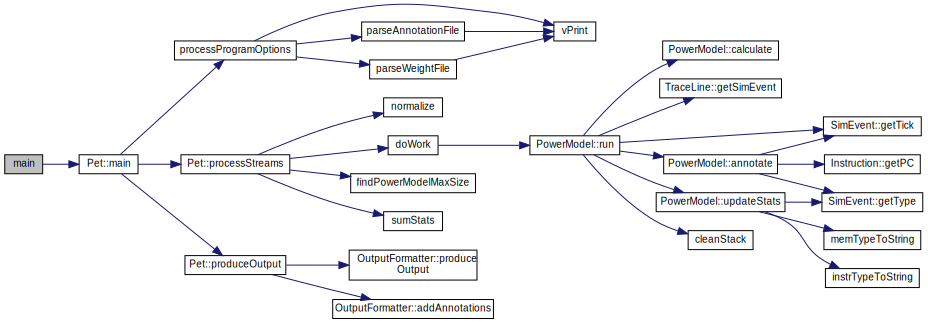
\includegraphics[width=\textwidth]{figs/maincallgraph.pdf}
    \caption{Call graph}
    \label{fig:callgraph}
\end{figure}



\subsection{Argument Parsing and Program Options}

As any other non-trivial programs, PET has to adapt to input options given from
the command line or from a settings-file. PET makes extensive use of the
\texttt{Boost}-library \cite{boostwebpage} and utilize
\texttt{Boost::Program\_options} for parsing the command line. Making use of
\texttt{Boost} for common tasks all over the program made the development cycle
less cumbersome and more rapid. \texttt{Boost::Program\_options} allows easy
extraction of program options, both with long (\texttt{\textemdash \textemdash
option=\emph{value}}) and short (\texttt{\textemdash o~\emph{value}})option
style.


\subsection{Reading Trace Logs}

When arguments are parsed and a trace log has been specified, either by path or
as \texttt{stdin}, a single thread is kicked off reading each line of the log
file into a C++ string container. This happens in the
\texttt{Pet::processStreams} method seen in \autoref{fig:callgraph}. The string
container is then inserted into one of many circular buffers. The circular
buffers are implemented with \texttt{boost::lockfree::spsc\_queue}, a lock free
single producer, single consumer queue. The property of beeing lock free is
explained by Tim Blechmann and the boost-community in \cite{boostlockfree} as
follows: "data structures are \emph{lock-free}, if some concurrent operations
are guaranteed to be finished in a finite number of steps. While it is in theory
possible that some operations never make any progress, it is very unlikely to
happen in practical applications". In PET, this queue has a fixed size of 8192,
but dynamic size is also available in the library implementation.

Which buffer the string is inserted into is determined by a simple circular
algorithm; the next ring buffer is selected when current one is full. When the
buffers are small enough to be filled fast enough to let all workers do work,
this method creates a lot less locking than using a single ring buffer shared by
all worker threads. The number of threads and the size of the ring buffers are
tightly coupled with how fast the host computer is able to feed PET with the log
files.

It is our experience that reading the log file is not the bottle neck, and it is
easy to feed at least 8 cores when the log file is hosted on a reasonable fast
drive. A simple benchmarking done with PET running on a system consisting of an
Intel Core i7 4820, 32GB DDR3 SDRAM and keeping the log files on a fake-RAID
Level-0 consisting of two Western Digital Caviar Black 750GB disks shows this.
PET running with 8 threads on this particular system is consuming the log files
with a rate of 133MB/s regardless of where the log files resides in RAM or on
disk. The benchmark used a log file of 5458MB and was run in 40.871 seconds.

\subsection{String to Event Mapping and Power Accumulation}

String parsing and mapping resembles the most compute-intensive parts of PET.
These parts of the program is kicked off as thread starting the
\texttt{doWork}-function, as the thread library cannot start running in methods
of instanceiated objects. As displayed in the callgraph in
\autoref{fig:callgraph}, this function simply starts the
\texttt{PowerModel::run}-method on its input, which an instance of the
PowerModel-class.

As the producer fills the ring buffers for each of the workers, the workers pick
strings from their pool. The strings are popped from the ring buffer, thus
making space for new elements right away. Each string is parsed by the TraceLine
class, which looks for patterns in the strings containing known event types.
When connecting PET with gem5, the trace logs as previously seen
\autoref{lst:trace} contains an event type designation in the second :-separated
column. The TraceLine class extracts this part using a very simple method to
make this part go fast, outline of this method is listed in
\autoref{alg:extract}.

\begin{algorithm}
    \begin{lstlisting}[style=algo,language=python]
function extractEventType( line ):
    start = line.find(":") + 1
    end = line.find(":", start)

    while (line[start] == ' ')
        start = from + 1
    while (line[end-1] == ' ')
        end = to - 1

    return line.substring(start, end)
    \end{lstlisting}
    \caption{Event Type Extraction}
    \label{alg:extract}
\end{algorithm}

In the real program, some more error handling is present, and the event types
are instanceiated as objects of their parent type (Instruction- or
Memory-event). The right parameters are further found from progressive string
parsing. If the event is not recognized, an "empty" object of type UnknownEvent
is returned, this type always has zero weight. Each event object is able to
figure out its own weight as written in the \emph{weights}-file. After the
event has been parsed, its weight is added to the power model at the right
time step.

In order to reduce the time used for disposal of the string objects
after they are parsed, they are places in a static-size array. When
this array is full, or the ring buffer is empty, the worker deletes
all the strings in a chunk. This methods keeps the memory footprint
low while not calling \texttt{free()} at a continuous rate. The \texttt{free()}
function is not considered very slow, but from the reference implementation
shown in \cite{kernighan1988c}, it does contain enough pointer
arithmetics to make a difference in a tight loop.

\subsection{Data Reduction}

When all lines from the trace log are consumed by the workers, the threads are
joined and their data is returned as standard C++-vectors. These result vectors
are further wrapped in yet another standard C++-vector. The inner vectors is
then looped over together, and the value from the current data point in each
vector is added together and put in a result vector. This accumulation happens
as the last part of \texttt{Pet::processStreams} as seen in
\autoref{fig:callgraph}. After a single point has been accumulated from the
vectors, idle time is calculated from how many events that was recorded during
the data point. This is done more simplistic than accurate using
\autoref{eq:idle}. $numEvents$ is the number of events recorded in each vector
at each measure point, and each event is pinned to the cycle where it
originated.

\begin{equation}
    totalEvents = \sum_{n=1}^{N} numEvents_n
\end{equation}
\begin{equation}
    idleEvents = \frac{ticksInDatapoint}{ticksInCycle}- totalEvents
\label{eq:idle}
\end{equation}

It should be noted that even though this method might work well in a
single-cycle in-order CPU, the out-of-order nature of the Cortex-A9 makes it
hard to tell how much idle time actually exists. E.g. A single cycle may fill
the pipeline with four events, then idle the three next cycles; this would be
calculated as no idle time. When the approximate numbers of \texttt{idleEvents} have been
estimated, that number is multiplied by the \emph{Idle}-weight and added to the
sum in the result vector. Finally, the entire vector is normalized according to
bucket size and then static current drain is applied.


\subsection{Output Production and Annotations}

After the result vector has been completely accumulated, annotation
is added to a new result vector in the same manner as the data reduction.
With the new, merged annotation map containing all last matches between
a symbol and the program counter within each measure point, this map
is feed to the \texttt{OutputProducer}-object as seen in \autoref{fig:callgraph}.
The \texttt{OutputProducer}-object is responsible for generating output as defined
by the input arguments. Its options have already been described in \autoref{sec:output},
and its implementation is a simple nested if-else-clause that calls internal functions for
each output type. The graphical output is produced using a wrapper around GNUPlot, while
the textual outputs are created by \texttt{printf}-statements.


\subsection{Unit Tests}

All internal string parsing are verified by unit tests. The unit tests
are written with help from the Boost Test Library Unit Test Framework \cite{boostunittest}.

The test library generates a new binary with the same program content, except the
main function, thus the program flow, is different. The test binary will
run through the listed functions with a certain input, and if the output is unexpected,
the test binary will print to the console an error message containing a description of what
went wrong. This approach helps refactoring and correctness in general, such that
the focus can be kept on the program surroundings.


\section{Input}
New hardware architectures are not easily analysed without physical
implementation, but often we are able to simulate its behaviour to acceptable
accuracy, and thus we are able to test different implementations with low cost.
These simulation runs can often be set up to produces trace logs which contains
a user controlled amount of detail. PET can use these trace logs and scan them
for predefined events, each affecting the power consumption of the simulated
hardware. Different simulators have different trace log formats and different
trace abilities. We have chosen gem5 as our target simulator as it is easy to
configure, and trace is well implemented. As mentioned in
\autoref{subsec:design_choises} other options are available, but the support for
easily configurable CPU- and memory system along with the pre-implemented ARM
processors and in-department hands-on experience with this simulator made gem5
the most logical choise.

\subsection{gem5 trace logs}
When run with \texttt{--debug-flags=Bus,Cache,MemoryAccess,Exec} gem5 will output trace files look like
the text displayed in \autoref{lst:trace}.

\begin{lstlisting}[basicstyle=\tiny,caption={gem5 trace log},label={lst:trace},escapeinside={@}{@},float]
@\label{line:physmem}@3021: system.physmem: Write of size 8 on address 0x82fe0 data 0xe1a0f00eee1d0f70
@\label{line:icache}@3021: system.cpu.icache: access for ReadReq address 9c0 size 64
@\label{line:cachemiss}@3021: system.cpu.icache: ReadReq (ifetch) 9c0 miss-
...
@\label{line:cacheupdate}@3432: system.cpu.dcache: Block addr 81f0 moving from state 0 to state:7 valid: 1
3432: system.cpu.dcache: Leaving recvTimingResp with ReadResp for address 81f00
3432: system.tol2bus.respLayer1: The bus is now busy from tick 234320 to 236376
@\label{line:memread}@1642: system.cpu T0 : 0x89d4.0 : ldr   r1, [sp] #4     : MemRead :  D=0x00000000
@\label{line:intalu}@1642: system.cpu T0 : 0x89d4.1 : addi_uop   sp, sp, #4 : IntAlu :  D=0x00000000b
1701: system.cpu T0 : 0x89d8   : mov   r2, sp          : IntAlu :  D=0x00000000b
1701: system.cpu T0 : 0x89dc.0 : str   r2, [sp, #-4]!  : MemWrite :  D=0x0000000
1760: system.cpu T0 : 0x89dc.1 : subi_uop   sp, sp, #4 : IntAlu :  D=0x00000000b
1760: system.cpu T0 : 0x89e0.0 : str   r0, [sp, #-4]!  : MemWrite :  D=0x0000000
4000: system.membus: recvTimingResp: src system.membus.master[0] ReadResp 0x1640
4000: system.l2: Handling response to ReadResp for address 1640
4000: system.l2: Block for addr 1640 being updated in Cache
\end{lstlisting}

Each line in \autoref{lst:trace} represents an event that happens in the
simulated hardware.  \autoref{line:physmem} tells that a write access to
physical memory has happened. \autoref{line:icache} is the event of instruction
cache access, while \autoref{line:cachemiss} shows that this request failed.
During this simulation, there is also events like \autoref{line:cacheupdate}
which represents that the data cache updates some content. The discrete
instructions running through the CPU is also logged, eg. \autoref{line:memread}
shows a load-instruction and \autoref{line:intalu} shows an
addition-instruction.

As discrete events are picked out from the trace logs, PET accumulates power
consumption in equally sized timeslots, called buckets. Each bucket has a
parameter controlled size in terms of simulator ticks. Often it is more
practical to specify the number of buckets in the output rather then specifying
the number of simulator ticks in each bucket. Because of this, PET is able to
estimate the bucket size by peeking at the tick at the last line of the trace
file. It has been shown that the trace file is not nessesary in tick order,
but it will commonly be at approximatly the last tick at the last line. The
bucket size estimation algorithm is shown in \autoref{alg:bucket_size}.

\begin{algorithm}
    \caption{Bucket Size Detection Algorithm}
    \label{alg:bucket_size}
    \begin{algorithmic}
        \Function{numTicks}{$traceFile$}

        \State $eofPos \gets \Call{getSize}{traceFile}$
        \State $\Call{seek}{traceFile, eofPos - 3}$
        \State
        \State $char \gets \Call{getChar}{traceFile}$
        \While{$char \ne newline$}
            \State $\Call{seek}{traceFile, -1}$
        \EndWhile
        \State $line \gets \Call{getLine}{traceFile}$
        \State $simulatorEvent \gets \Call{parseLine}{line}$
        \State \Return $\Call{getTick}{simulatorEvent}$
        \EndFunction
    \end{algorithmic}
    \begin{lstlisting}[language=Python]
function numTicks( traceFile ):
    # Find file size
    eof_pos = traceFile.getSize()

    # Seek almost to end, avoid last newline
    traceFile.seek( eof_pos - 3 )

    # Trace from back of file to second last newline
    while not traceFile.currentChar is '\n':
        traceFile.seek_backwards

    # File stream position is now at beginning of last line
    # Parse this line
    simulatorEvent = parseLine( traceFile.getLine() )

    # Return the tick of the retreived event
    return simulatorEvent.getTick()
    \end{lstlisting}
\end{algorithm}

\autoref{lst:trace} also shows that the events in the trace log is not nessesary in their
correct order, thus PET has to be able to add power consumption to the entire timeline at all
time. This means that we are unable to produce continous output, but have to store the
results in memory and dump them when the entire input is parsed.


\subsection{PET weight files}
Equally important as finding the correct events is assigning each event the
correct amount of power consumption. As each event will count differently
depending on the architecture, PET will read a weight file along with the gem5
trace log. A sample weight file is listed out in \autoref{lst:weights_example}.
As the timeslots are specified in simulator ticks instead of CPU cycles,
the values have been chosen to match a 2GHz processor, which then means
one CPU cycle pr. 500 simulator ticks using standard gem5 simulation granularity.
If you are applying this method to a processor with a different clock speed than
2GHz, be aware that the numbers has to be scaled propotionally. This is not the
case for the static power drain, as it is simply added to each timeslot, and is
not scaled in accordance with bucket size.

\lstinputlisting[caption={Weight file example},label={lst:weights_example},float,language=Python]{examples/weights.conf}

The weights displayed in \autoref{lst:weights_example} are assigned and
accumulated each time PET discovers a recognisable event in the log file. A
simplified version of this algorithm can be found in
\autoref{alg:power_accum_algo}

\begin{algorithm}
\caption{Power Accumulation Algorithm}
\label{alg:power_accum_algo}
\begin{lstlisting}[language=Python]
# map of accumulated power for each time step
map<time,power> output

# input is all trace log lines, elements in weight file and
# the determined bucket size (number of simulator ticks in
# each bucket)

function assignWeights( traceLogLines, weightMap, bucketSize )
    # run through each line
    for each line in traceLogLines:
        # extract event parameters from line
        simulatorEvent = parseLine( line )

        # get the assigned weight from weight file
        eventWeight = weightMap[simulatorEvent.getEventType()]

        # add this weight to the output map
        output[simulatorEvent.getTick()/bucketSize] += eventWeight
    return output
\end{lstlisting}
\end{algorithm}
%weightfiles
%

\subsection{Annotation files}
\label{subsec:annot}
PET has the ability to annotate it's output using a map from PC to function name. The
simulated binary itself is not an input to PET, as it would contain to much information to display nicely in
an ordinary graph. Instead, PET comes along with a tool called \texttt{scripts/annotate.sh} which takes
a binary file as input and prints out all function names in the binary file. The binary file must be compiled
with debugging symbols for this to work. The usual situation would then be to pull out those function names you want
to annotate be editing the output from this tool, and then giving this file to PET as annotation input.

An example of how this map can look like is printed in \autoref{lst:annot}. The
left column is simply the PC value where the function label points, and the
right column is the function name.
\lstinputlisting[caption={Annotation file example},label={lst:annot},float,language=Python]{examples/annot.conf}

\section{Output}
\label{sec:output}

When a log file is consumed by PET, the output should be usable for many
applications. In early stages of the design phase, or when great differences are
expected, a sparse annotated graphical output might be the best way of
visualizing power consumption. As the project evolves and more subtle changes
are evaluated, a textual output will be easier to compare. PET supports three
different output options:

\begin{description}
    \item[graph]\hfill\\
        This format is the default, and provides an overview of
        the entire program in an easily digestible format. An example of such
        a graph is printed in \autoref{fig:annot}.
    \item[plain]\hfill\\
        The example in \autoref{lst:pet_output_plain} shows the \emph{plain}
        format, which is intended to be used for further machine processing.
    \item[table]\hfill\\
        The table format, with an example shown in
        \autoref{lst:pet_output_table}, shows a terminal-printable output which
        is easier to read. It might come in handy as the default format might be
        hard to read when you are looking for specific information.
\end{description}

\subsection{Units}

The output format is understood as timeslots in which the architecture has a
certain current drain, which should be multiplied with applied voltage to get
consumed energy. The values are given as milliamperes, equal to milliwatt if
voltage is $1~V$. Milliamperes are used as it is easier to find current drain
rather than wattage with the setup used in this project, as described in
\autoref{sec:energymeasure}. When power is estimated for a new architecture, the
resistance of the circuit is difficult to deduce, and voltage might also be an
unknown factor. Given Ohms law in \autoref{eq:ohm} and the definition of
electric power in \autoref{eq:power}

\begin{equation}
I=\frac{U}{R}
\label{eq:ohm}
\end{equation}

\begin{equation}
P=U \cdot I
\label{eq:power}
\end{equation}

it can be found that power equals current squared times resistance

\[U=R \cdot I\]
\[P=(R \cdot I) \cdot I\]
\begin{equation}
P=I^2 \cdot R
\label{eq:currentsquared}
\end{equation}
and that power equals voltage squared divided by resistance
\[P=U \cdot \frac{U}{R}\]
\begin{equation}
P=\frac{U^2}{R}
\label{eq:voltagesquared}
\end{equation}

Thus, estimating only the current drain means that the power at each point will
be unknown without knowing resistance or voltage. Further, energy consumption
cannot be estimated unless the new architecture is similar in terms of voltage
and resistance to a chip where these numbers are available. Even the current
drain might not be representable at all; if resistance or voltage is unequal to
the levels found in the reference chip, the final numbers will be far off.

\autoref{eq:currentsquared} and \autoref{eq:voltagesquared} states how voltage
and current is important for energy consumption. The current is, from
\autoref{eq:ohm}, dependent on resistance as well as voltage. With this in mind,
and knowing that power in a complex environment is a delicate matter, the most
important application for PET is to point in the right direction. PET will never
give accurate power estimations for new chips, but will provide useful
information for seeing if a new feature or architectural fix will render the
final architecture more energy efficient or not.


\subsection{Examples of Output Data}

Visualization is often a good thing when inspecting old or trying to understand
new problems. \autoref{fig:annot} shows an example of PET \texttt{graph} output
format, with annotations.

\begin{figure}[htb]
    \centering
    \includegraphics[width=0.9\textwidth]{figs/annot.pdf}
    \caption{PET graphical output. This example contains annotations, each label
    represents the entrance of a function.}
    \label{fig:annot}
\end{figure}

Example of the \texttt{plain} output format can be seen in
\autoref{lst:pet_output_plain}. The left column is the bucket number, while the
right column is instant current draw from the modeled architecture.

\begin{lstlisting}[numbers=none,float=hbt,label={lst:pet_output_plain},caption={PET plain output with function annotations.}]
0 120 memcpy
1 113 start
2 150 main
3 123 main
4 133 fun1
5 117 main
\end{lstlisting}

When reading the output directly from console, a more descriptive output format
is the \texttt{table} format. An example using this option is rendered in
\autoref{lst:pet_output_table}.

\begin{lstlisting}[numbers=none,float=hbt,label={lst:pet_output_table},caption={PET table output with function annotations.}]
/----------------------------------------\
|   Bucket   |  milliAmps |    Symbol    |
|------------|------------|--------------|
|          0 | 120.000000 |    memcpy    |
|          1 | 113.000000 |    start     |
|          2 | 150.000000 |    main      |
|          3 | 123.000000 |    main      |
|          4 | 133.000000 |    fun1      |
|          5 | 117.000000 |    main      |
\----------------------------------------/
\end{lstlisting}




usage
- input-format, input-parameter
- kjøring av gem5, flagg, se-mode
- (kryss)-kompilering av test-programmer
output
- plain, table, graph
- annotering (med eksempler på hvordan man får tak i dette)
